%% Chapter01-绪论.tex
%% 绪论
\chapter{绪论}

\section{基本概念}
\begin{itemize}
    \item \textbf{激光成像}:Laser Imaging, LI.
    \item \textbf{激光遥感}:Laser Remote Sensing, LRS.
    \item \textbf{激光雷达}:Light Detection And Ranging, LiDAR.
    \item \textbf{机载激光地形测绘}:Airborne Laser Terrain Mapping, ALTM.
    \item \textbf{机载激光制图}:Airborne Laser Mapping, ALM.
    \item \textbf{机载激光扫描}:Airborne Laser Scanning, ALS.
    \item \textbf{机载激光测高}:Airborne laser altimetry, ALA.
    \item \textbf{激光测高}:Laser Altimetry, LA.
    \item \textbf{机载激光扫描测高}:Airborne Laser Scanning Altimetry, ALSA.
    \item \textbf{空载光达、空载雷射扫描}:Light Detection And Ranging, LiDAR.
\end{itemize}

\section{应用现状}
\begin{enumerate}
	\item % 森林检测与管理
	\textbf{森林检测与管理}。LiDAR系统的最早商业应用领域之一。\\
	\textbf{传统技术}:以前是借助空中摄影和地面测量进行的。这些方法不仅费时费力,而且只能分析样点,结果还是推断的。\\
	\textbf{激光雷达的优势}:激光扫描法能克服这些缺点,通过激光扫描技术
	提取得完整的3D森林模型。在单个树木分析的基础上,可确定以下的参数:\begin{itemize}
		\item 单个树高
		\item 一片林区的平均树高
		\item 一片林区的木材体积
		\item 一片林区的平均密度
		\item 每片林区的平均生长体积
	\end{itemize} 
	此外LiDAR得到的DTM还可以来规划和改善森林运输道路,以及进行倾斜度分析,以便测定危险。
	\item % 构建数字城市模型
	\textbf{构建数字城市模型}:
	在电信、无线通讯、法律实施和灾难管理等众多领域中都需要准确的数字城市模型(建筑物建模、城市规划、噪声模拟、无线网络规划)
	\item % 湿地、限制进入地区、危险区域
	\textbf{湿地、限制进入地区、危险区域}
	\begin{itemize}
		\item 密集的植被覆盖和没有可通行的道路。
		\item 传统的地面摄像测量技术很难对沼泽、野生动物保护区及森林保护区进行勘测。
		\item 危险地带的地貌特征获取。
	\end{itemize}
	\item \textbf{油气管道勘测}
	\item \textbf{洪水灾情预测}(洪水制图、灾害评估)获取流域的数字表面模型和数字高程模型。
	\item \textbf{海岸线监测与制图}
	\item \textbf{水深、海岸线、侵蚀状况监测}
	\item \textbf{电力线监测}
	\item \textbf{股文物保护}
	\item \textbf{真正射影像的制作}
\end{enumerate}

\section{LiDAR技术特点}
\begin{enumerate}
	\item 无需光照条件或专门的太阳高度角。
	\item 可在白天、夜晚或相当恶劣的条件下(大雾)作业,全天时全天候获取地面三维数据。
	\item 能部分“穿透”植被,同时测量地面和非地面层。
	\item 很少需要进入测量现场,不需要大量的地面控制点。
	\item 能快速获取数据,24小时内可提取测区的DEM数据。
	\item 精度较高。
	\item 能够接受无穷次回波。
	\item 可在地面反射率比较低的区域工作,例如反射率只有约5\%的地面。
	\item 集成RS和GPS技术,数据可直接作为GIS的数据源,有利于提高地理数据的自动化,加快处理速度。
	\item 一个飞行日内可采集高达200 GB的数据。
	\item 高速度、高性能、高精度、长距离的航空测量设备。
	\item 全数字化,可直接产生三维坐标$ (X,Y,Z) $,无需其他额外步骤。
	\item 数据密集。基于固定翼机载平台采集时,典型的激光光斑中心间距为0.5 m左右。
	\item 精度:针对地物建模应用情形,典型精度达15 cm。
	\item 机载平台:便于操作,易于快速获取地表数据。
	\item 宽视场角:最大可以达到$ 75^{\circ} $的视场角。如果部分视场角范围没有被用到,可以用于飞机倾角稳
	定补偿。
\end{enumerate}

\section{激光成像技术}
\subsection{激光}
\paragraph{地位}\textit{激光}是20世纪以来,继原子能、计算机、半导体之后,人类的又一重大发明,被称为“最快的刀”、“最准的尺”、“最亮的光” 。
\paragraph{激光的亮度}约为太阳光的100亿倍。
\paragraph{激光的特点} \begin{itemize}
	\item 单色性、方向性、相干性
	\item 具有很高的单光子辐射能量
	\item 在大气传输中很少发生绕射
\end{itemize}
\paragraph{激光设备}1960年发明\textit{红宝石激光器},主要在军事上得到了应用。\begin{itemize}
	\item \textbf{激光测距仪}:美国1969年测地月距离。
	\item \textbf{激光致盲器}:1982年英阿马岛战争投入实战。
	\item \textbf{激光制导器}:1991年海湾战争,精度高、抗干扰能力强。
	\item \textbf{激光告警设备、激光干扰设备}等电子战装备。
\end{itemize}
\paragraph{激光的应用}\begin{itemize}
	\item \textbf{自然科学}
	\item \textbf{加工领域}
	\item \textbf{信息处理}
	\item \textbf{激光通信}
	\item \textbf{医学领域}
	\item \textbf{测绘领域}
	\item \textbf{环境检测}:弥补了微波在绕射和不能探测目标生化特性的不足,有了更加广泛的应用范围。 \begin{itemize}
		\item 大气成分探测(气溶胶探测)
		\item 污染探测大气和海洋基本参数,如:海水深度、温度等探测。
		\item 绿色植物探测
	\end{itemize}
\end{itemize}
\paragraph{微波雷达的局限性}\begin{itemize}
	\item 其波长较长,相应能量子的能量很小。
	\item 一般不足以与目标发生生化作用,无法探测目标的生化特性。
	\item 在传播过程中,遇到尺寸小于波长的物体时,更易于发生衍射。
\end{itemize}
\subsection{激光雷达与激光成像雷达}
\paragraph{激光雷达的光源类型}\begin{itemize}
	\item 可见光波段{\kaishu \ce{He}-\ce{Ne}和\ce{Ar}激光器}
	\item 短波红外波段{\kaishu Nd:YAG激光器}。最成熟的激光器。
	\item 长红外波段的{\kaishu \ce{CO2}激光器}。正在研制的大多是\ce{CO2}激光器,体积大,价格比较高。
	\item \textit{二极管泵浦固体激光雷达}(DPL),20世纪80年代后期。是发展重点。\\
	\textbf{DPL的优点}:\begin{itemize}
		\item 无需制冷
		\item 不像红外热成像系统容易受环境影响
		\item 对人眼安全,大气消光比低
		\item 可采用光纤光路和集成光学技术
		\item 结构小型化,体积小,制作成本低
		\item 具有高稳频、高功率、高效率和高光束质量等优点
		\item 可距离成像和强度成像
	\end{itemize}
	\textbf{DPL与其他激光器的比较}:\begin{itemize}
		\item \textbf{与Nd:YAG激光器相比}:后者只能测距和测角,不能测速,成像困难,大气传输性较差。
		\item \textbf{与\ce{CO2}激光器相比}:相干性好,寿命长,可靠性强。
	\end{itemize}
	\textbf{DPL的应用}\begin{itemize}
		\item 军事的应用
		\item 大气测污、风场测量、环境监测
	\end{itemize}
\end{itemize}
\paragraph{激光成像雷达的基本结构} 如图\ref{fig:激光成像雷达的基本结构}所示。
\begin{figure}[htbp]
	\centering
	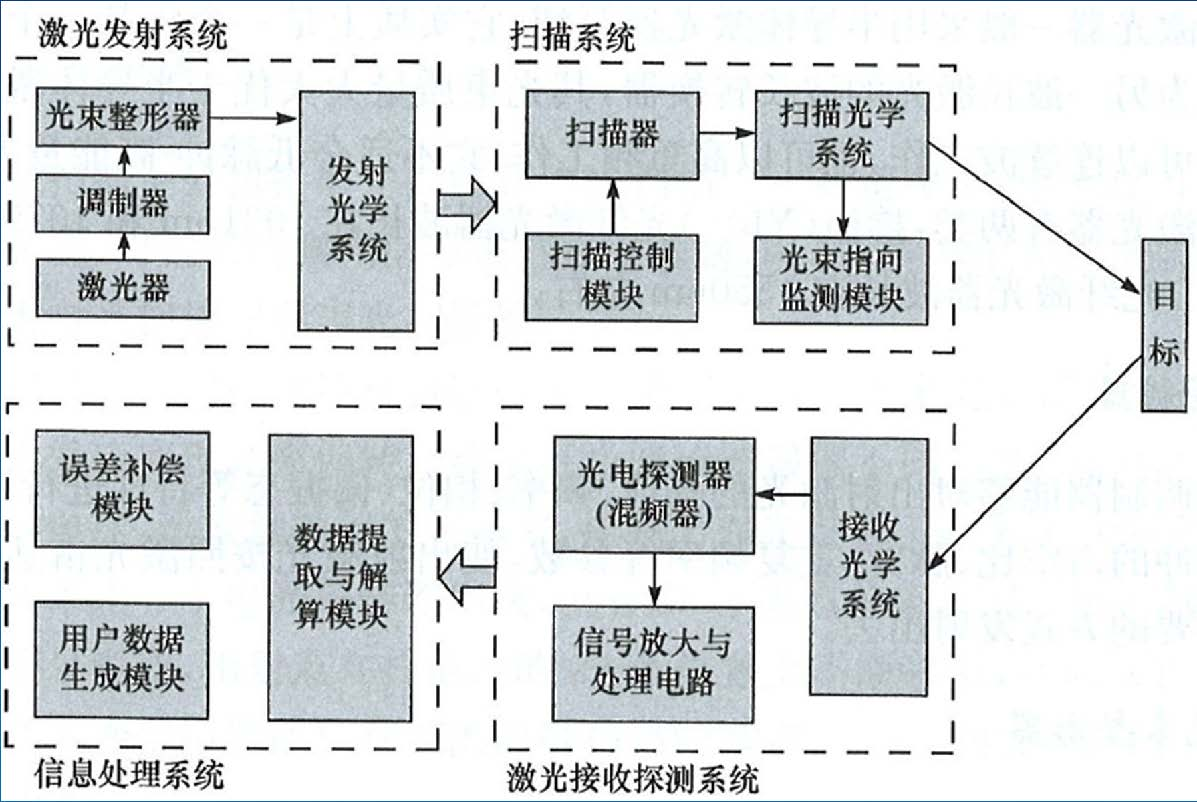
\includegraphics[width=0.7\linewidth]{figure/Chapter1/激光成像雷达的基本结构.jpg}
	\caption{激光成像雷达的基本结构}
	\label{fig:激光成像雷达的基本结构}
\end{figure}
\paragraph{激光成像雷达的发展}
\begin{itemize}
	\item 20世纪70年代,卫星激光测距(阿波罗登月计划)
	\item 1980至1988,机载LiDAR可行性研究。
	\item 1990年,斯图加特大学研制成功首个激光断面测 量系统
	\item 1993年,德国出现首个商用LiDAR系统TopScan(ALTM 1020)
	\item 1995年,全球有5套商用LiDAR系统
	\item 1999年,全球约有30几套商用LiDAR系统
	\item 2001年,全球约有75个公司使用了60几套商用LiDAR系统
	\item 2002年,全球约有120个公司使用了75几套商用LiDAR系统 ,年平均增长率为7.1\%,市场份额从5\%增长到12\%。
	\item 目前国内已引进20余套机载激光雷达系统。
\end{itemize}
\paragraph{激光雷达的新类型}\begin{enumerate}
	\item \textit{扫描激光雷达}\begin{itemize}
		\item 扫描成像激光雷达在对地观测领域最为成熟的应用是机载LiDAR系统。
		\item 采用单元探测器,每次测量只获得一个像素的数据,通过平台运动和扫描实现一定探测范围的成像。
		\item 机载LiDAR系统一般采用脉冲激光体制,要求激光的重复频率高,脉冲宽度窄,单脉冲能量大。
		\item 由记录的距离数据形成的图像称为距离图像,由记录的回波强度数据形成的图像称为强度图像。
	\end{itemize}
	\item \textit{凝视激光雷达(新型)}\\
	\textbf{原理}:凝视成像激光雷达需要控制发射激光,使发射光覆盖整个成像区域,然后通过面阵探测器接收回波,通过飞行时间测量或调制解调手段实现并行测距,得到目标三维图像。\\
	\textbf{优点}:凝视成像激光雷达实现了“瞬时”成像,具有结 构简单、成像速率高、像素分辨率高等诸多优点,有着广阔的应用前景。
	\item \textit{合成孔径激光雷达(新型)}\\
	\textbf{原理}:原理与微波合成孔径雷达类似,不同的是辐射源采用了激光波段。在距离向上发射大时宽带宽信号,对回波信号进行脉冲压缩得到距离向高分辨率;方位向上利用雷达平台与目标之间的相对运动,记录平台不同位置的目标回波信号,经相关的数据处理在空间上合成一个虚拟的大孔径,实现方位向聚焦,获得方位向的高分辨率。\\
	\textbf{优点}:合成孔径激光雷达是一种新型的主动式激光成像 雷达,它综合了传统的微波合成孔径雷达和激光雷达的优势。突破实孔径的衍射极限,当观测距离达到数百公里甚至更远时,它是唯一能够在有限的光学孔径条件下获得厘米级分辨率的光学成像手段。
\end{enumerate}

\subsection{激光雷达的关键技术}
下列四项技术中,前三项属于硬件技术,均已得到不同程度的解决;第四项技术属于软件技术,目前成为最关键的技术。
\begin{enumerate}
	\item \textit{激光发射器}:高功率和高波束质量的辐射源
	\begin{enumerate}
		\item \textit{气体激光器}\\	%% 气体激光器
		\textbf{特点}:\begin{itemize}
			\item 典型的气体激光器为\ce{CO2}
			\item 最早用于激光雷达的激光器之一
			\item 工作波长为10.6 \textmu m,处于大气窗口。
			\item 至今仍广泛用于激光雷达
		\end{itemize}
		\textbf{优点}:\begin{itemize}
			\item 大气传输性能好,效率高。
			\item \ce{CO2}激光雷达易于实现高灵敏度外差探测和三维成像,信息处理技术成熟。
		\end{itemize}
		\textbf{缺点}:\begin{itemize}
			\item 尺寸比较大
			\item 需要低温制冷
		\end{itemize}
		\item \textit{固体激光器}:应用非常广泛的Nd:YAG激光器 \begin{itemize}
			\item 在典型情况下,脉宽10~30 ns,单脉冲能量为100 mJ~1 J,脉冲重复率为10~100 Hz。
			\item 波长1.06 \textmu m的基频辐射YAG激光器可用于研究大气散射。
			\item 波长0.532 \textmu m的2倍频频光可用于海洋勘探。
			\item 波长0.355 \textmu m和0.266 \textmu m的3倍频和4倍频光可用于测污
		\end{itemize}
		\item \textit{半导体二极管激光器},又称半导体激光器又称激光二极管。\\ %% 半导体二极管激光器
		是用半导体材料作为工作物质的激光器。常用工作物质有砷化镓(\ce{GaAs})、硫化镉(\ce{CdS})、 磷化铟(\ce{InP})、硫化锌(\ce{ZnS})等。\\
		激励方式有电 注入、电子束激励和光泵浦三种形式。\\
		\textbf{特点}:半导体二极管激光器是最实用最重要的一类激光器。它体积小、寿命长,并可采用简单的注入电流的方式来泵浦其工作电压和电流与集成电路兼容,因而可与之单片集成。\\
	\end{enumerate}
	\item \textbf{成像探测器}:高灵敏度接收技术。\\ %% 成像探测器
	\textit{成像探测器}也称光电探测器(或混频器),是指将望远镜接收到的激光信号,直接转换成与之对应的电信号,或者将光信号与本振光混频,实现外差探测并将其转换成电信号。\\
	目前激光雷达采用的主流探测器包括:\textit{光电倍增管}(PMT)、\textit{雪崩光电二极管}(APD)、PIN\textit{光电二极管}、\textit{增强型电荷耦合器件}(ICCD)。\\
	激光雷达探测系统所采用的探测器一般有三种类型:\begin{enumerate}
		\item \textit{单元探测器}:\begin{itemize}
			\item 每次只获得一个像素的数据。
			\item 激光器每次发出宽度很窄的脉冲(一般以纳秒计)。
			\item 回波强度反映了目标的反射率特性。
			\item 使用扫描器控制发射脉冲按一定方式扫描,将光束指向不同目标,或目标上的不同位置。
			\item 通过接收系统形成图像,距离数据形成的图像称为距离图像,回波强度数据形成的图像称为强度图像。
			\item 要求激光重复频率高,脉冲宽度窄,单脉冲能量大。
			\item 激光成像雷达的高成像速率和高分辨率常常不能同时得到满足,采用单元探测器时,这一矛盾更加突出,所以需要折中考虑。
		\end{itemize}
		\item \textit{面阵探测器}:\begin{itemize}
			\item 需要控制发射激光,使发射光能覆盖较大面积的目标或同时照射许多不同的目标,然后接收回波信号。
			\item 需要对发射光进行调制,对接收信号进行解调,才能量测出距离。
			\item 不需要扫描器,但要求发射功率大。
			\item 无法采用高灵敏度的探测器。
			\item 在希望成像像素数多,成像速率要求不高的情况下采用。即在成像速率要求不高,成像分辨率要求很高的情况下采取的一种办法。
		\end{itemize}
		\item \textit{阵列探测器}:受限于器件技术以及信号处理技术水平,阵列探测器经历了单元模块阵列化、PIN阵列探测、APD阵列探测,及从线阵到面阵的发展阶段。\begin{itemize}
			\item \textbf{线阵探测}:需要将发射光分为$ N $束,同时照射目标上的$ N $点,从这些点上反射回来的信号由$ N $个探测元所接收,得到$ N $个像素上的距离信息和强度信息;
			\item 通过扫描器扫描,获得二维信息,对扫描器的要求比较高;
			\item 可以实现高速高分辨率成像。
			\item 技术难度较大
		\end{itemize}
	\end{enumerate}
	\item \textbf{扫描系统}:高性能二维扫描技术。用于激光成像雷达系统的扫描器目前可分为三种:力学、电学和二元光学扫描。
	\begin{enumerate}
		\item \textit{力学扫描器}:由反射镜转动或摆动使光束偏转进行大角度范围扫描。结构如图\ref{fig:力学扫描器结构}所示。
		\begin{figure}[htbp]
			\centering
			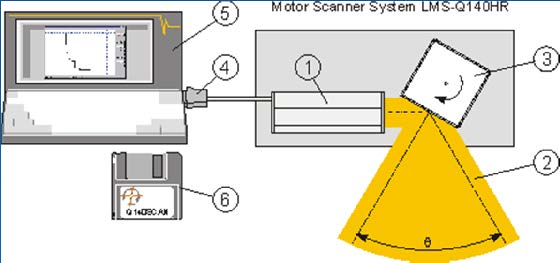
\includegraphics[width=0.7\linewidth]{figure/Chapter1/力学扫描器结构}
			\caption{力学扫描器结构}
			\label{fig:力学扫描器结构}
		\end{figure}\\
			\textbf{优点}:采用转镜可以达到很高的扫描速度,两个转镜可组成二维扫描系统。\\
			\textbf{缺点}:体积较大,笨重,耗电量大。
		\item \textit{声光电学扫描器}:\\
			\textbf{优点}:不包含机械运动,扫描速度快。\\
			\textbf{缺点}:\begin{itemize}
				\item 扫描角度小,一般为几十分之一毫弧度。
				\item 光透过率低,光束质量差。
				\item 耗电量大,光学系统必须作冷却处理。
			\end{itemize}
		\item \textit{二元光学扫描器}:利用二元光学技术制造,通过两组透镜的相对移动实现光束方向的偏转。\\
		\textbf{原理}:利用二元光学技术制造出来的微透镜阵列扫描器由间距只有几微米的微透镜阵列组成,分为两组:一组是正透镜,一组是负透镜。准直光经过透镜时会会聚光,然后通过负透镜时又变为准直光。正透镜阵列和负透镜阵列之间产生相对移动时,准直光的方向就会发生变化。两个微透镜阵列在水平方向相对移动时,输出光束在水平方向就会发生偏转。透镜之间微小的相对移动可以产生几度的光束偏转。\\
		\textbf{优点}:\begin{itemize}
			\item 扫描速度可以达到1KHz以上。
			\item 易于将一束光分为多束光。
			\item 扫描方式可通过编程任意加以改变。
			\item 体积小,重量小。
		\end{itemize}
		\textbf{缺点}:\begin{itemize}
			\item 但扫描角度较小,透过率较低。
			\item 尚未实用。
		\end{itemize}
	\end{enumerate}
	\item \textbf{数据处理技术}:图像处理及目标识别算法
\end{enumerate}

\section{激光遥感集成系统}
\paragraph{激光成像雷达的不足}虽然,激光成像雷达可以获取目标高精度的三维信息(包含高程信息和强度信息),但
\begin{itemize}
	\item 集成GPS/INS方可获取地标目标的绝对位置。
	\item 光谱、纹理信息缺乏,不利于地物识别。
\end{itemize}
\paragraph{激光遥感集成系统}随着数码相机等硬件技术的发展,将数码相机、GPS/INS与激光雷达集成,提高激光雷达的数据获取能力,已成为当前激光雷达系统获取数据的主要方式。(图\ref{fig:激光遥感集成系统})
\begin{figure}[htbp]
	\centering
	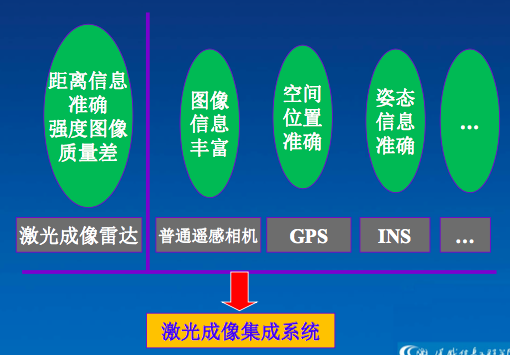
\includegraphics[width=0.7\linewidth]{figure/Chapter1/激光遥感集成系统}
	\caption{激光成像集成系统}
	\label{fig:激光遥感集成系统}
\end{figure}
\paragraph{激光遥感观测系统}由以下部分组成
\begin{itemize}
	\item 飞机
	\item 激光扫描仪
	\item 航摄相机
	\item 导航控制系统
	\item 高精度位置姿态测量系统(IMU/DGPS)
	\item IMU与相机连接架
	\item 机载DGPS天线
	\item 地面DGPS基站接收机
\end{itemize}
\paragraph{激光遥感集成系统的发展}\begin{enumerate}
	\item 美国航空航天局(NASA)最早支持开发激光成像三维测量的机载集成系统。
	\item 加拿大、瑞典、德国以及中国也相继开发出这类机载集成系统,可用于陆地和浅海水下地形测量。
\end{enumerate}
\section{国内常见LiDAR系统的扫描方式}
\paragraph{摆镜扫描}Leica、Optech采用的扫描方式。如图\ref{fig:摆镜扫描方式}所示。
\begin{figure}[htbp]
	\centering
	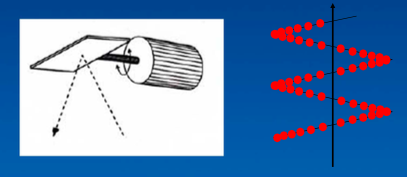
\includegraphics[width=0.7\linewidth]{figure/Chapter1/摆镜扫描方式}
	\caption{摆镜扫描方式图示}
	\label{fig:摆镜扫描方式}
\end{figure}
\paragraph{旋转棱镜扫描}Toposys Harrier、Riegl、IGS采用。如图\ref{fig:旋转棱镜扫描方式}所示。
\begin{figure}[htbp]
	\centering
	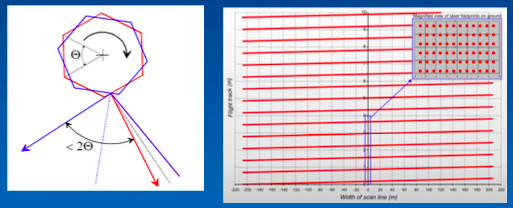
\includegraphics[width=0.7\linewidth]{figure/Chapter1/旋转棱镜扫描方式}
	\caption{旋转棱镜扫描方式}
	\label{fig:旋转棱镜扫描方式}
\end{figure}
\paragraph{光线扫描方式}Toposys Falcon系列。如图\ref{fig:光纤扫描方式}所示。
\begin{figure}[htbp]
	\centering
	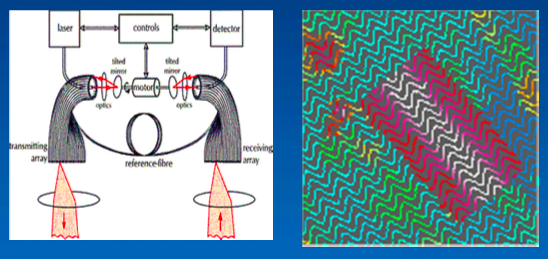
\includegraphics[width=0.7\linewidth]{figure/Chapter1/光纤扫描方式}
	\caption{光纤扫描方式}
	\label{fig:光纤扫描方式}
\end{figure}
\paragraph{圆锥镜扫描方式}opEye MK 系列、国产三维激光成像仪采用。如图\ref{fig:圆锥镜扫描方式}所示。
\begin{figure}[htbp]
	\centering
	\subfloat[圆锥镜扫描原理]{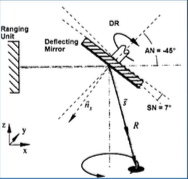
\includegraphics[width=0.5\linewidth]{figure/Chapter1/圆锥镜扫描_原理}}
	\subfloat[圆锥镜扫描脚点形状]{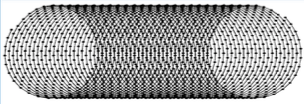
\includegraphics[width=0.8\linewidth]{figure/Chapter1/圆锥镜扫描_脚点}}
	\caption{圆锥镜扫描方式}。
	\label{fig:圆锥镜扫描方式}
\end{figure}
\section{机载激光三维测量系统对比}
如图\ref{fig:机载激光三维测量系统对比}。
\begin{figure}[!htbp]
	\centering
	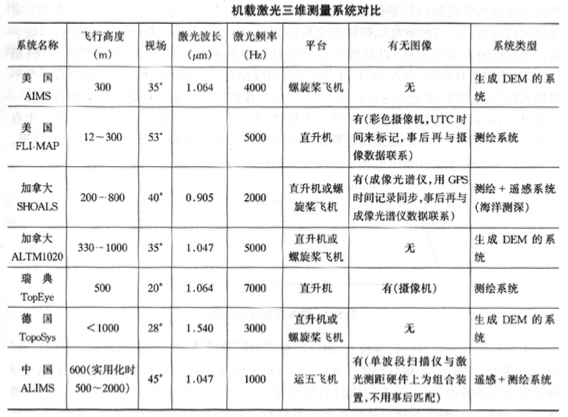
\includegraphics[width=1\linewidth]{figure/Chapter1/机载激光三维测量系统对比}
	\caption{机载激光三维测量系统对比}
	\label{fig:机载激光三维测量系统对比}
\end{figure}
